\documentclass[prodmode,acmtecs]{acmsmall} % Aptara syntax

% Package to generate and customize Algorithm as per ACM style
\usepackage[ruled]{algorithm2e}
\usepackage{graphicx}
\usepackage{float}
\usepackage{comment}
\usepackage{amsmath}
\usepackage{amssymb}

\renewcommand{\algorithmcfname}{ALGORITHM}
\SetAlFnt{\small}
\SetAlCapFnt{\small}
\SetAlCapNameFnt{\small}
\SetAlCapHSkip{0pt}
\IncMargin{-\parindent}

% Metadata Information
\acmVolume{1}
\acmNumber{1}
\acmArticle{1}
\acmYear{2016}
\acmMonth{12}

% Copyright
\setcopyright{rightsretained}

% Document starts
\begin{document}

% Title portion
\title{Favorite Stock Filter}
\author{Jaehoon Kim
\affil{Drexel University}
Junbang Huang
\affil{Drexel University}}

\begin{abstract}
Recurrent Neural Network has been well understood in handling 
Time series data. Different from feedforward neural networks, 
recurrent neual network has internla memory to process temporal
related sequences of inputs. However, not all recurrent neural network
can handle "long-term" dependencies. The reasons are explored in depth
by Hochereiter (1991) [German] and Bengio, et al. (1994). In our project, we 
use Long Short Term Memory network - usually just called "LSTMs" to model
Time series data. Unlike other RNN, LSTMs are explicityly designed to avoid the 
long-term dependency problem. In this paper, we will show how LSTMs are used 
to train a model that can handle real-world stock data of 200 weeks in temporal length. 
The model classify stock into two class. One is manipulated and the other is 
non manipulated. Through carefully designed training, the cross validation 
shows that our model has a accuracy of 80\% ~ 90\%. We also observed that 
the accuracy drops when iterations we used to train our data increased. 
Besides, cost drops as the number of iterations increase. 
\end{abstract}

\ccsdesc[500]{Computer Science~Machine Learning}
\ccsdesc[500]{Machine Learning~Neural Network}
\ccsdesc[500]{Machine Learning~Recurrent Neural Network}
\ccsdesc[500]{Machine Learning~Long Short Term Memory RNN}

%
% End generated code
%

\terms{Machine Learning, Deep Learning, Neural Network, Algorithms, Performance}

\keywords{Recurrent Nueral Network, LSTM RNN, Time series modeling, cross validation, tensorflow, tensorboard}

\maketitle

\newpage
\section{Background}

\subsection{The goal of the project}
As the development of computer science and computer enginerring, our computer, or 
system, to be more accurate, runs faster than ever before. Trading firm takes advantage of 
this. Due to this reason, high performance trading has been created, which relies on high 
performance computing and low latency system to provide very important trading information 
and help traders make trading decisions. \\\\
One of the simplest trading strategy is investing the safe stocks. So what is safe stocks? 
Safe stocks are manipulated stocks. Because they are manipulated, they tend to have a safe line 
and a foreseeable peak value. Traders can make safe decision by investing in manipulated stocks 
when their prices are near the safe line and sell stocks when they are closing to highest value. \\\\
The goal of this project is to train a model that can classify "good" stock and "bad" stock, and therefore, 
can be used to help all investor to make decision wisely.

\subsection{Challenges}
There are two big challenges we are facing during this project. They are both caused by one thing,
that is the input data. 

\begin{itemize}
\item Stock data is time series data. Time series data add extra 
difficulties in how to handle it. Unlike normal data, time series mean that the next 
value in a time serie is affected by the previous one. We know that we can train 
neural networks with historical data and objective to discover hidden dependencies and 
to predict stock type. Therefore, to solve this problem, we need to answer this question 
that how can we model time series?
\item Another problem is that stock prices vary from each other. Some stocks rage from 
0 ~ 10, some range from 0 ~ 100. Due to this reason, we had difficulty to understand the outcome 
of our model. Since we are not sure whether we train the model in a correct way, it costed us a very 
long to figure out where went wrong. The solution is simple, normalizing input data.
\end{itemize}

\newpage
\section{Related Work}
To implement our model, we read many useful article, paper and blogs. The following are 
summaries of some of them. The others will be mentioned as references at the bottom of the paper.

\subsection{Recurrent neural networks, Time series data and IoT - Part One [Ajit Jaokar]}
This blog explores the relationship between recurrent neural networks (RNNs) and IoT data (Time series data). \\
There are two parts that are very helpful for us to implement our mode. Therefore, I only mention those two important parts here. \\ Firstly, why Time Series applications are different. In our case, Time Series applications mean prediction application that uses Time series data to predict the future value. Different from calssical pattern recognition problems, who are more concerned with knowing dependencies between variables (Regression) or in classification of input vectors into categories (Classification). The biggest difference is that time series data has an additional temporal dimension. \\ Secondly, why neural networks can be used. Neural networks are a strong choice when we have scenarios that there are too many factors influencing the outcome, and that there are hidden/unknown factors influencing the outome. In such case, the focus is not to find the precise solution to the problem but to find a possible steady where the system will converge. Neural networks often apply in such cases for the reason that they are able to learn from history examples and are able to catch hidden dependencies. \ Therefore, the problem becomes how can we model Time in the neural network.

\subsection{Understandling LSTM Networks}
The previous post points an direction for us, which is we need to find appropriate neural network to model time series data. This post talks about one type of the Recurrent Neural Network, which is LSTM Networks. It is a perfect neural network for our project. \\
Why Recurrent Neural Networks can model time series data? One of the major shortcoming of traditional neural networks is that they are unable to model time series data. However, Recurrent neural networks can address this issue. They do it using loops to create memory to remember information. Traditional neural network takes input data, put them through hidden layers and get outcome. After every iteration, weights between input-hidden and hidden-output will change in order to get a better result of the guessing. The major different differences between recurrent neural network and traditional neural network is that, RNN has one more step, that is there is a loop, allowing information to be passed from one step of the network to the next. If we unroll the recurrent neural network, we can easily notice that they are naturally related to sequences and lists. Therefore, they are a very good fit for time series data.\\
Are they really able to connect previous information to the present task? It depends on how far we look back for previous information. Sometimes, we only need recent information. Sometimes, we need information that is far back from now. Unfortunately, as the gap between the relevant information and the point where it is needed to becomes larger, RNNs become unable to learn to connect the information.\\
Luckly, Long Short Term Memory networks can addres such problem. Remembering information for long periods of time is their default behavior! The main idea of LSTM network is that it contains LSTM blocks that can remember a value for an arbitrary length of time.

\newpage
\section{Approch}
\label{sec:sim}
This section describes theories and concepts used in the project

\subsection{Basic concept of recurrent neural network (RNN)}
RNN is a neural network but RNN has two input: one is from data, another is from previous output. Usually RNN is used with serial data. For example, human language sentence has series of words and data has time domain like driving data and stock data.

\subsection{Long Short Term Memory (LSTM) networks}
Basic RNN has problem of long term dependency \cite{UnderstandingLSTMNetworks}. It means that RNN is not able to memorize long term knowledge. To solve the problem, LSTM is introduced by Hochreiter and Schmidhuber \cite{hochreiter1997long}. LSTM has cell state and the cell state can store long term memory. LSTM has four layer and three of them effect to cell state. Colah's blog \cite{UnderstandingLSTMNetworks} summarizes concept and purpose of each layers. The paper \cite{zaremba2014recurrent} describes LSTM in mathematical term. In this paper, I'm going to summarize the blog \cite{UnderstandingLSTMNetworks} and the paper \cite{zaremba2014recurrent}

\begin{enumerate}
	\item Concept of each layers in LSTM\\
		Bengio mentioned on his paper \cite{bengio2009learning} that each layers in deep neural network have purpose. LSTM has four layers and four layers have different purpose. Colah's blog \cite{UnderstandingLSTMNetworks} summarizes it.\\
		The first layer is forget gate and effects to cell state and filters what data to forget or throw away. This layer is sigmoid layer with previous output and input data. The second layer is input gate and also effects to cell state and it decides what data to remember. The second layer is also sigmoid. The third layer is input modulation gate and also effects to cell state and it is tanh. Out put from second and third layers are added to previous cell state and updated for next cell state. Fourth layer is the last layer output gate and output is decided from result of output gate and updated cell state.

	\item Modeling LSTM in mathematical term\\
		LSTM is described in mathematical term in the paper \cite{zaremba2014recurrent}. I'm going to summarize it on this paper.\\
		Let\\
		$T_{n,m}: \mathbb{R}^n \rightarrow \mathbb{R}^m$ be an affine transform\\
		$x_t$ be current input \\
		$h_{t-1}$ be last output \\
		$h_{t}$ be current output \\
		$c_{t-1}$ be last cell state \\
		$c_{t}$ be current cell state \\
		
\[
\begin{bmatrix}
    input gate \\
    forget gate \\
    output gate \\
    input modulation gate
\end{bmatrix}
=
\begin{bmatrix}
    i \\
    f \\
    o \\
    g
\end{bmatrix}
=
\begin{bmatrix}
    sigm \\
    sigm \\
    sigm \\
    tanh
\end{bmatrix}
T_{2n,4n}
\begin{bmatrix}
    h_{t-1} \\
    x_{x}
\end{bmatrix}
\]
\[
=
\begin{bmatrix}
    sigm \\
    sigm \\
    sigm \\
    tanh
\end{bmatrix}
\begin{bmatrix}
    {T^{hi}}_{n,n} & {T^{xi}}_{n,n} \\
    {T^{hf}}_{n,n} & {T^{xf}}_{n,n} \\
    {T^{ho}}_{n,n} & {T^{xo}}_{n,n} \\
    {T^{hg}}_{n,n} & {T^{xg}}_{n,n}
\end{bmatrix}
\begin{bmatrix}
    h_{t-1} \\
    x_{x}
\end{bmatrix}
=
\begin{bmatrix}
    sigm \\
    sigm \\
    sigm \\
    tanh
\end{bmatrix}
\begin{bmatrix}
    {T^{hi}}_{n,n}h_{t-1} + {T^{xi}}_{n,n}x_{x} \\
    {T^{hf}}_{n,n}h_{t-1} + {T^{xf}}_{n,n}x_{x} \\
    {T^{ho}}_{n,n}h_{t-1} + {T^{xo}}_{n,n}x_{x} \\
    {T^{hg}}_{n,n}h_{t-1} + {T^{xg}}_{n,n}x_{x}
\end{bmatrix}
\]
Multiply two vector not matrix multiplication. Therefore,\\
\[
\begin{bmatrix}
    i \\
    f \\
    o \\
    g
\end{bmatrix}
=
\begin{bmatrix}
    sigm({T^{hi}}_{n,n}h_{t-1} + {T^{xi}}_{n,n}x_{x}) \\
    sigm({T^{hf}}_{n,n}h_{t-1} + {T^{xf}}_{n,n}x_{x}) \\
    sigm({T^{ho}}_{n,n}h_{t-1} + {T^{xo}}_{n,n}x_{x}) \\
    tanh({T^{hg}}_{n,n}h_{t-1} + {T^{xg}}_{n,n}x_{x})
\end{bmatrix}
\]

$\{i, f, o, g\}$ is a set of output from each layers.
The current cell state $c_t = f \cdot c_{t-1} + i \cdot g$
the current output $h_t = o \cdot tanh(c_t)$

\end{enumerate}

\subsection{LSTM in Stock Filter}
Our project uses LSTM to filter data. We created LSTM with size of 32 hidden layer. That means size of cell state and output is 32. After we map 200 weeks, we take last output from LSTM them map output layer. Output layer has two neurons and make result by using softmax. Following picture describes neural network

\begin{figure}[H]
	\begin{center}
	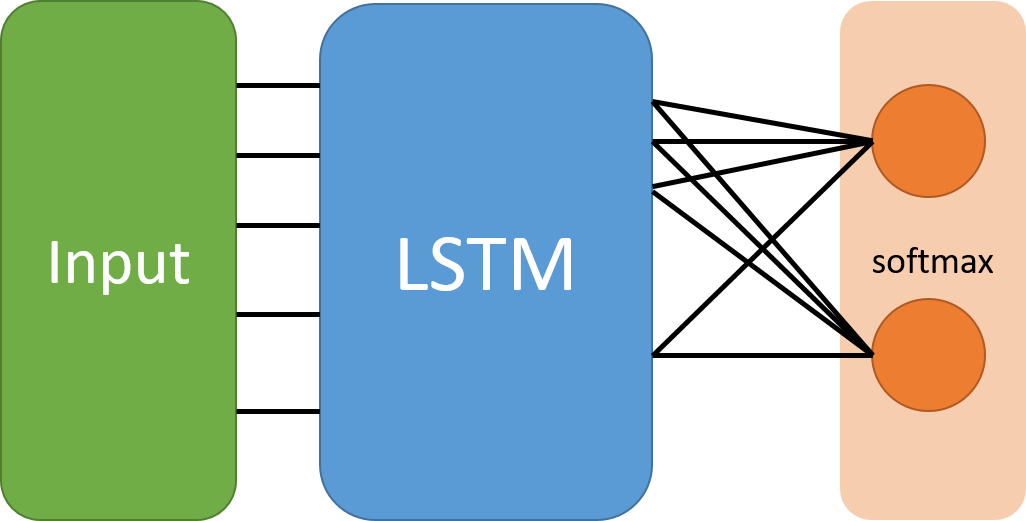
\includegraphics[scale=0.7]{./pictures/FSFNN.png}
	\caption{High Level Neural Network}
	\label{GD}
	\end{center}
\end{figure}

\newpage
\section{Evaluation}
\subsection{Data}
\begin{enumerate}
	\item Features in stock data\\
		Stock data has 7 features: date, open, high, low, close, volumn, and adj close. Date is when stock data is recorded. Open price is stock price when market open. Close price is when market close. High price is the highest price during market time and low is the lowest price during market time. However, we only use 5 features: high, low, close, volumn because we do not need date and adj close price. 
		
	\item 200 Weekly data\\
		To classify stocks, each stock should have enough data. In the project, we use 200 weekly data from each stock. 200 weeks is almost 4 years data.
		
	\item Class\\
		Stocks in our data are divided to two groups: like and dislike. Stock market trader gave the data for the project. We assume that stocks in like group are effected by some big money so the stocks has supported line and stocks in dislike group does not have support line. 
\end{enumerate}

\subsection{Data}

\subsection{Data}

\newpage
\section{Conclusions}
In this article, we develop the first multifrequency MAC protocol for
WSN applications in which each device adopts a
single radio transceiver. The different MAC design requirements for
WSNs and general wireless ad-hoc networks are
compared, and a complete WSN multifrequency MAC design (MMSN) is
put forth. During the MMSN design, we analyze and evaluate different
choices for frequency assignments and also discuss the nonuniform
back-off algorithms for the slotted media access design.
\\
\\
\\
\section{Future Work}
The following are future works. There are two parts, one is samll updates and changes. The second part is about making it an stand alone API.
\subsection{Small Improvements}
\begin{enumerate}
\item Current, we are using weekly stock data to train and test our mode. Which means our model only support weekly stock data. Our next improvement is obivous, that is to support daily and yearly stock data for the reason that yearly and daily stock data are also very common.
\item The second improvement is to support dynamic time frame. Currently, we are using fixed temporal length of stock data, which is 200 weeks in temporal length. The limitation of fixed length is that not all stock is published for that long. With the support of dynamic time frame, we can analysis all stock theoretically. 
\item Only classifying stocks may not be usful. Even with a "good" stock at hand, many people still do not know how to do. The best way is to tell people when to buy which one. In other to do that, we need to train a model to detect increase signal. 
\end{enumerate}

\subsection{Stand alone API}
We can always improve our model. As shown above, there are three interesting changes that we really want to make. However, there is one that is really big that prepares our project to be a very usful one, that is making it aa stand alone API. The following steps to achieve this goal.
\begin{enumerate}
\item Like other API, people can use it without caring about its implementation. All they care is accuracy. Since accuracy is taken care through this paper, I will skip this part. In this case, the first thing to make it an API, we need to implement interfaces that people can use it.
\item Although users do not care about the detail implementation, we do care about it a lot. There are two things that we care about. System availability and computing power. Yes, we can make it as a system that is used as very simple API by users. To deal with availability and computing power, we can use distributed system skills. For example, there are many great systems that we can learn from. Cassandra, Spark, and Redis. I will skip the deal here, since I need a book to talk about those issues. To sum up, the idea is that it can be a system that provides high quality and easy-to-use service for other people.
\end{enumerate}

\newpage
\bibliographystyle{plain}
\bibliography{references.bib}


\end{document}
% End of v2-acmsmall-sample.tex (March 2012) - Gerry Murray, ACM


